\begin{question}%[codigo:EAM200501AMX; concurso:EAM; ano:2005; assunto:; alternativa:]
Um cavalo deve ser amarrado a uma estaca situada em um dos vértices de um pasto que tem a forma de um quadrado, cujo lado mede 20m. Para que ele possa pastar em cerca de 20\% da área total do pasto, a parte inteira, em metros, do comprimento da corda que o prende á estaca deve ser igual a
    \begin{tasks}
        \task \(1\).
        \task \(2\).
        \task \(5\).
        \task \(8\).
        \task \(10\).
    \end{tasks}
\end{question}

\begin{question}%[codigo:EAM200502AMX; concurso:EAM; ano:2005; assunto:conjuntos, conjuntos numéricos; alternativa:]
Dado o seguinte problema: "Subtraindo-se \(3\) de um certo número \(x\), obtém-se o dobro da sua raiz quadrada. Qual é esse número?"; pode-se afirmar que, no conjunto dos números reais, esse problema
    \begin{tasks}
        \task tem duas soluções.
        \task tem só uma solução, a que é um número primo.
        \task tem só uma solução, a que é um número par.
        \task tem só uma solução, a que é um número ímpar e não primo.
        \task não tem solução.
    \end{tasks}
\end{question}

\begin{question}%[codigo:EAM200503AMX; concurso:EAM; ano:2005; assunto:geometria; alternativa:]

% \begin{figure}[h!]
    % 
    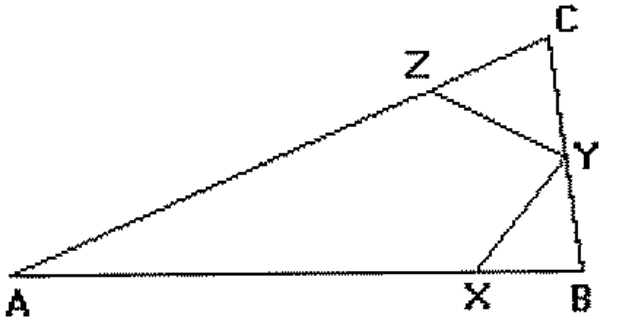
\includegraphics[width=.3\textwidth]{CONCURSO/EAM/IMAGES/2005/EAM200503IMG.png}
% \end{figure}


Na figura acima, \(AB = AC\), \(BX = BY\) e \(CZ = CY\). Se o ângulo \(A\) mede \(40^\circ\), quanto mede o ângulo \(XYZ\)?
    \begin{tasks}
        \task \(40^\circ\).
        \task \(50^\circ\).
        \task \(60^\circ\).
        \task \(70^\circ\).
        \task \(90^\circ\).
    \end{tasks}
\end{question}

\begin{question}%[codigo:EAM200504AMX; concurso:EAM; ano:2005; assunto:trigonometria no triângulo,trigonometria; alternativa:]

% \begin{figure}[h!]
    % 
    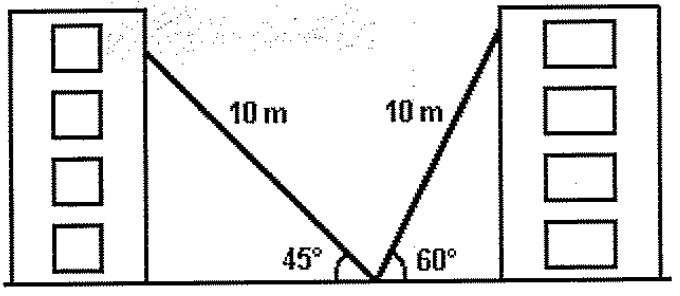
\includegraphics[width=.3\textwidth]{CONCURSO/EAM/IMAGES/2005/EAM200504IMG.png}
% \end{figure}

Uma escada de 10 metros de comprimento forma ângulo de \(60^\circ\) com a horizontal quando encostada ao edifício de um dos lados da rua, e ângulo de \(45^\circ\) se for encostada ao edifício do outro lado, apoiada no mesmo ponto do chão. A largura da rua, em metros, vale aproximadamente
    \begin{tasks}
        \task \(15\).
        \task \(14\).
        \task \(13\).
        \task \(12\).
        \task \(11\).
    \end{tasks}
\end{question}

\begin{question}%[codigo:EAM200505AMX; concurso:EAM; ano:2005; assunto:; alternativa:]
Uma balança assinala 325g para um certo copo cheio de água. Jogando-se metade da água fora, a balança passa a assinalar 180g. Para esse copo vazio, quanto tal balança assinalará em gramas?
    \begin{tasks}
        \task 20.
        \task 25.
        \task 35.
        \task 40.
        \task 45.
    \end{tasks}
\end{question}

\begin{question}%[codigo:EAM200506AMX; concurso:EAM; ano:2005; assunto:; alternativa:]
Numa competição de tiro-ao-alvo, cada atirador deve efetuar \(25\) disparos. Qual a porcentagem de acertos no alvo de um jogador que obtém \(+0,5\) pontos, sabendo-se que cada tiro no alvo vale \(+0,4\) e cada tiro fora do alvo vale \(-0,1\)?
    \begin{tasks}
        \task \(25\).
        \task \(24\).
        \task \(20\).
        \task \(16\).
        \task \(5\).
    \end{tasks}
\end{question}

\begin{question}%[codigo:EAM200507AMX; concurso:EAM; ano:2005; assunto:; alternativa:]
Um feirante compra duas unidades de maça por R\$ 0,75. Sabendo-se que ele vende o lote de seis maças por R\$ 3,00, quantas maças deverá vender para ter um lucro de R\$ 50,00?
    \begin{tasks}
        \task 50.
        \task 52.
        \task 400.
        \task 520.
        \task 600.
    \end{tasks}
\end{question}

\begin{question}%[codigo:EAM200508AMX; concurso:EAM; ano:2005; assunto:geometria,área de figuras; alternativa:]

% \begin{figure}[h!]
    
    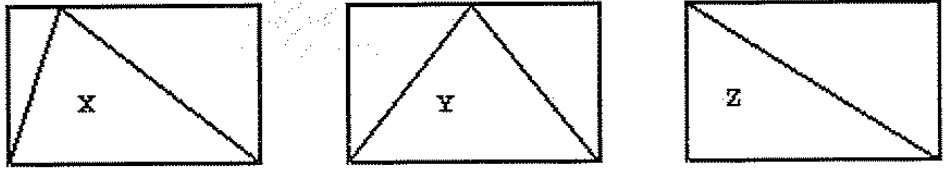
\includegraphics[width=.5\textwidth]{CONCURSO/EAM/IMAGES/2005/EAM200508IMG.png}
% \end{figure}

Considerando-se que, nas figuras acima, os triângulos \(X,Y\) e \(Z\) estejam inscritos em retângulos congruentes, pode-se afirmar que
    \begin{tasks}
        \task apenas as áreas dos triângulos \(X\) e \(Y\) são iguais.
        \task apenas as áreas dos triângulos \(X\) e \(Y\) são iguais.
        \task apenas as áreas dos triângulos \(Y\) e \(Z\) são iguais.
        \task as áreas dos triângulos \(X,Y\) e \(Z\) são iguais entre si.
        \task as áreas dos triângulos \(X, Y\) e Z são diferentes entre si.
    \end{tasks}
\end{question}

\begin{question}%[codigo:EAM200509AMX; concurso:EAM; ano:2005; assunto:múltiplos; alternativa:]
Numa unidade da Marinha, estão lotados: 200 terceiros sargentos; 160 segundos sargentos; e \(n\) primeiros sargentos. Se \(n\) representa \(2/5\) do número total de sargentos da referida unidade, pode-se afirmar que \(n\)
    \begin{tasks}
        \task é múltiplo de 15 e de 8.
        \task é múltiplo de 15 e não de 8.
        \task não é múltiplo de 15, nem de 8.
        \task não é múltiplo de 15, mas é múltiplo de 8.
        \task é múltiplo de 18.
    \end{tasks}
\end{question}

\begin{question}%[codigo:EAM200510AMX; concurso:EAM; ano:2005; assunto:; alternativa:]
Em uma sala retangular de piso plano nas dimensões 8,80m por 7,60m, deseja-se colocar lajotas quadradas iguais sem a necessidade de recortar qualquer peça. A medida máximo, em centímetros, do lado de cada lajota deverá ser igual a
    \begin{tasks}
        \task 10.
        \task 20.
        \task 30.
        \task 40.
        \task 50.
    \end{tasks}
\end{question}

\begin{question}%[codigo:EAM200511AMX; concurso:EAM; ano:2005; assunto:; alternativa:]
Fatorando-se a expressão \(ac + 2bc - ad -2bd\), obtém-se
    \begin{tasks}
        \task \((a+2b)(c-d)\).
        \task \((a-2b)(c-d)\).
        \task \((a-2b)(c+d)\).
        \task \((a+c)^2(a-d)\).
        \task \((a-c)(a+2b)\).
    \end{tasks}
\end{question}

\begin{question}%[codigo:EAM200512AMX; concurso:EAM; ano:2005; assunto:; alternativa:]
Caso seja cobrado um imposto de 5\% sobre o valor de qualquer saque efetuado em uma instituição financeira, qual será o saque máximo possível, em reais, a ser efetuado em uma conta cujo saldo é de 2 100,00 reais?
    \begin{tasks}
        \task 1 995,00.
        \task 2 000,00.
        \task 2 050,00.
        \task 2 075,00.
        \task 2 095,00.
    \end{tasks}
\end{question}

\begin{question}%[codigo:EAM200513AMX; concurso:EAM; ano:2005; assunto:volume; alternativa:]
A maquete de um reservatório \(R\), feita na escala \(1:500\), tem 8mm de largura, 10mm de comprimento e 8mm de altura. Qual é a capacidade em litros do reservatório \(R\)?
    \begin{tasks}
        \task 640.
        \task 800.
        \task 6400.
        \task 8000.
        \task 80000.
    \end{tasks}
\end{question}

\begin{question}%[codigo:EAM200514AMX; concurso:EAM; ano:2005; assunto:trângulo; alternativa:]
Em um triângulo, os lados medem 9cm, 12cm e 15cm. Quanto mede, em centímetros, a altura relativa ao maior lado desse triângulo?
    \begin{tasks}
        \task 8,0.
        \task 7,2.
        \task 6,0.
        \task 5,6.
        \task 4,3.
    \end{tasks}
\end{question}

\begin{question}%[codigo:EAM200515AMX; concurso:EAM; ano:2005; assunto:perímetro; alternativa:]

% \begin{figure}[h!]
    
    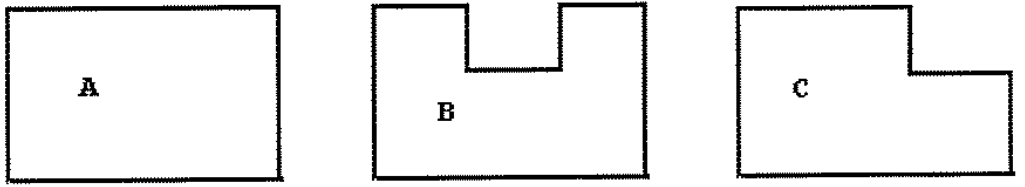
\includegraphics[width=.5\textwidth]{CONCURSO/EAM/IMAGES/2005/EAM200515IMG.png}
% \end{figure}

Considerando-se que a figura \(A\) seja um retângulo e as figuras \(B\) e \(C\) sejam obtidas, respectivamente, pela retirada da figura \(A\) de um quadrado de lado unitário, pode-se afirmar que
    \begin{tasks}
        \task apenas os perímetros das figuras \(A\) e \(B\) são iguais.
        \task apenas os perímetros das figuras \(A\) e \(C\) são iguais.
        \task apenas os perímetros das figuras \(B\) e \(C\) são iguais.
        \task os perímetros das figuras \(A,B\) e \(C\) são todos iguais.
        \task os perímetros das figuras \(A,B\) e \(C\) são todos diferentes.
    \end{tasks}
\end{question}
